\documentclass{standalone}
\usepackage{fontspec}
\setsansfont{DejaVuSans.ttf}[Path=./,Kerning=Off,Ligatures={TeXOff,NoCommon}]
\usepackage{tikz}
\begin{document}
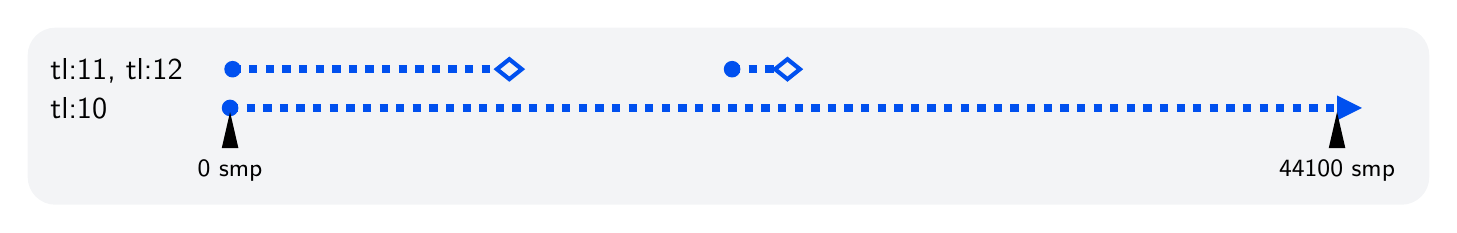
\begin{tikzpicture}[x=1pt,y=1pt,miter limit=4,font=\sffamily]
\definecolor{ts000000}{HTML}{000000}
\definecolor{ts0050EF}{HTML}{0050EF}
\definecolor{tsF3F4F6}{HTML}{F3F4F6}
\begin{scope}[shift={(16,16)}]
\path[rounded corners=10pt,fill=tsF3F4F6] (0,0) rectangle (506.4678,63.9766);
\path[draw=ts0050EF,line width=3pt,dash pattern=on 3pt off 3pt] (73.1377,34.9766) -- (473.1377,34.9766);
\path[fill=ts0050EF] (73.1377,34.9766) circle[radius=3];
\path[fill=ts0050EF] (482.1377,34.9766) -- (473.1377,39.4766) -- (473.1377,30.4766) -- cycle;
\path[draw=ts0050EF,line width=3pt,dash pattern=on 3pt off 3pt] (74.0447,48.9766) -- (169.5447,48.9766);
\path[fill=ts0050EF] (74.0447,48.9766) circle[radius=3];
\path[draw=ts0050EF,line width=1.5pt] (169.5447,48.9766) -- (174.0447,52.5766) -- (178.5447,48.9766) -- (174.0447,45.3766) -- cycle;
\path[draw=ts0050EF,line width=3pt,dash pattern=on 3pt off 3pt] (254.5436,48.9766) -- (270.0436,48.9766);
\path[fill=ts0050EF] (254.5436,48.9766) circle[radius=3];
\path[draw=ts0050EF,line width=1.5pt] (270.0436,48.9766) -- (274.5436,52.5766) -- (279.0436,48.9766) -- (274.5436,45.3766) -- cycle;
\path[fill=ts000000] (73.1377,33.4766) -- (70.1377,20.4766) -- (76.1377,20.4766) -- cycle;
\path[fill=ts000000] (473.1377,33.4766) -- (470.1377,20.4766) -- (476.1377,20.4766) -- cycle;
\node[anchor=base west,inner sep=0,font=\sffamily\fontsize{11}{12.8047}\selectfont,text=ts000000] at (8,45.1685) {tl:11, tl:12};
\node[anchor=base west,inner sep=0,font=\sffamily\fontsize{11}{12.8047}\selectfont,text=ts000000] at (8,31.1685) {tl:10};
\node[anchor=base,inner sep=0,font=\sffamily\fontsize{9}{10.4766}\selectfont,text=ts000000] at (73.1377,10.1226) {0 smp};
\node[anchor=base,inner sep=0,font=\sffamily\fontsize{9}{10.4766}\selectfont,text=ts000000] at (473.1377,10.1226) {44100 smp};
\end{scope}
\end{tikzpicture}
\end{document}
